\section{Analysis}
\subsection{Risk analysis}

\paragraph{Methodology}
We identify risks that could affect the implementation of the UI framework and the use cases. Each risk has a probability of occurrence as shown in table \ref{tab:probability} and a severity as explained in table \ref{tab:severity}. Multiplication of both scores yields the risk factor. We list all risks sorted descending by their risk factor in table \ref{tab:riskanalysis}. A risk factor greater or equal \textbf{8} indicates a risk that is likely to cause substantial project damage. \\
Furthermore, decisions that are made in section \ref{sec:proofofconcept} are based on this sorted list of risks.

\begin{table}[!htb]
  \begin{center}
    \begin{tabular}{|l|l|l|}
      \hline
      \textbf{Probability} & \textbf{Score} & \textbf{Description} \\
      \hline
      0 <= p <= 0.25 & 1 & The probability of occurrence of this risk is minimal. \\
      \hline
      0.25 < p <= 0.5 & 2 & The risk might occur with a low probability. \\
      \hline
      0.5 < p <= 0.75 & 3 & There is a significant chance for the risk to occur. \\
      \hline
      0.75 < p <= 1 & 4 & The probability of occurrence of this risk is high. \\
      \hline
    \end{tabular}
    \caption{The probability of occurrence is mapped to a score which is used in the risk analysis.}
    \label{tab:probability}
  \end{center}
\end{table}

\begin{table}[!htb]
  \begin{center}
    \begin{tabular}{|l|l|l|}
      \hline
      \textbf{Severity} & \textbf{Score} & \textbf{Project Damage} \\
      \hline
      insignificant & 1 & \begin{tabular}[x]{@{}l@{}}It is possible to implement the UI framework and the use cases \\ but the results might be poor.\end{tabular} \\
      \hline
      moderate & 2 & \begin{tabular}[x]{@{}l@{}}It is possible to implement the UI framework and the use cases \\ but the results might be unusable.\end{tabular} \\
      \hline
      high & 3 & \begin{tabular}[x]{@{}l@{}}It is possible to implement the UI framework and the use cases. \\ That approach to UI development is less efficient and more \\ costly than UI development without the UI framework.\end{tabular} \\
      \hline
      fatal & 4 & \begin{tabular}[x]{@{}l@{}}It is not possible to implement the UI framework and the use cases. \\ The thesis is neither confirmed nor rejected and no value is generated.\end{tabular} \\
      \hline
    \end{tabular}
    \caption{The level of severity is mapped to a score which is used in the risk analysis.}
    \label{tab:severity}
  \end{center}
\end{table}

\begin{table}[!htb]
  \begin{center}
    \begin{tabular}{|l|l|}
      \hline
      \textbf{ID} & R1 \\
      \hline
      \textbf{Title} & Incomplete HATEOAS specification \\
      \hline
      \textbf{Probability of occurrence} & 2 \\
      \hline
      \textbf{Severity} & 4 \\
      \hline
      \textbf{Risk Factor} & 8 \\
      \hline
      \textbf{Description} & \begin{tabular}[x]{@{}l@{}}The HATEOAS specification in use is either an early draft or it \\ has been abandoned. In the worst case the specification superficially \\ appears to be complete while not providing crucial features that \\ are needed by the use cases. Parts of it have to be written during the \\ thesis work.\end{tabular} \\
      \hline
    \end{tabular}
    \caption{Source of risk R1.}
  \end{center}
\end{table}

\begin{table}[!htb]
  \begin{center}
    \begin{tabular}{|l|l|}
      \hline
      \textbf{ID} & R2 \\
      \hline
      \textbf{Title} & Unstable HATEOAS specification and tooling\\
      \hline
      \textbf{Probability of occurrence} & 3 \\
      \hline
      \textbf{Severity} & 1 \\
      \hline
      \textbf{Risk Factor} & 3 \\
      \hline
      \textbf{Description} & \begin{tabular}[x]{@{}l@{}}The HATEOAS specification in use and reference implementations \\ are under development and parts are rewritten frequently. For the \\ thesis work a version has to be pinpointed.\end{tabular} \\
      \hline
    \end{tabular}
    \caption{Source of risk R2.}
  \end{center}
\end{table}

\clearpage

\begin{table}[!htb]
  \begin{center}
    \begin{tabular}{|l|l|}
      \hline
      \textbf{ID} & R3 \\
      \hline
      \textbf{Title} & Lack of HATEOAS tooling \\
      \hline
      \textbf{Probability of occurrence} & 2 \\
      \hline
      \textbf{Severity} & 2 \\
      \hline
      \textbf{Risk Factor} & 4 \\
      \hline
      \textbf{Description} & \begin{tabular}[x]{@{}l@{}}The HATEOAS specification in use has no reference implementation, \\ little working examples and no tools for generating and consuming \\ HATEOAS APIs. All tools have to be written from scratch.\end{tabular} \\
      \hline
    \end{tabular}
    \caption{Source of risk R3.}
  \end{center}
\end{table}

\begin{table}[!htb]
  \begin{center}
    \begin{tabular}{|l|l|}
      \hline
      \textbf{ID} & R4 \\
      \hline
      \textbf{Title} & Lack of JSON-LD tooling \\
      \hline
      \textbf{Probability of occurrence} & 1 \\
      \hline
      \textbf{Severity} & 3 \\
      \hline
      \textbf{Risk Factor} & 3 \\
      \hline
      \textbf{Description} & \begin{tabular}[x]{@{}l@{}}There are no tools that implement the JSON-LD operations \\ discussed in section \ref{jsonld}. The used languages and frameworks don't \\ support JSON as first class citizen. All tools have to be written \\ from scratch.\end{tabular} \\
      \hline
    \end{tabular}
    \caption{Source of risk R4.}
  \end{center}
\end{table}

\begin{table}[!htb]
  \begin{center}
    \begin{tabular}{|l|l|}
      \hline
      \textbf{ID} & R5 \\
      \hline
      \textbf{Title} & Lack of design language implementations \\
      \hline
      \textbf{Probability of occurrence} & 1 \\
      \hline
      \textbf{Severity} & 4 \\
      \hline
      \textbf{Risk Factor} & 4 \\
      \hline
      \textbf{Description} & \begin{tabular}[x]{@{}l@{}}The UI framework provides usable UIs out of the box. These  \\ are created by using a design language implementation which \\ takes care of portability across browsers. The implementation provides \\ the authors with best practices in UI design and layout. In case \\ there is a lack of design language implementations one has to \\ be written from scratch.\end{tabular} \\
      \hline
    \end{tabular}
    \caption{Source of risk R5.}
  \end{center}
\end{table}

\clearpage

\begin{table}[!htb]
  \begin{center}
    \begin{tabular}{|l|l|}
      \hline
      \textbf{ID} & R6 \\
      \hline
      \textbf{Title} & Linked data-driven UIs are slow \\
      \hline
      \textbf{Probability of occurrence} & 3 \\
      \hline
      \textbf{Severity} & 4 \\
      \hline
      \textbf{Risk Factor} & 12 \\
      \hline
      \textbf{Description} & \begin{tabular}[x]{@{}l@{}}JSON-LD operations as discussed in section \ref{jsonld} require multiple \\ requests per user request. This adds some overhead to \\ the client-server communication which can decrease performance. \\ If those additional requests can not be mitigated by caching, the \\ overhead might affect the UX. \end{tabular} \\
      \hline
    \end{tabular}
    \caption{Source of risk R6.}
  \end{center}
\end{table}

\begin{table}[!htb]
  \begin{center}
    \begin{tabular}{|l|l|l|}
      \hline
      \textbf{ID} & \textbf{Risk Factor} & \textbf{Title} \\
      \hline
      \rowcolor{red}
      R6 & 12 & Linked data-driven UIs are slow \\
      \hline
      \rowcolor{yellow}
      R1 & 8 & Incomplete HATEOAS specification \\
      \hline
      R5 & 4 & Lack of design language implementations \\
      \hline
      R3 & 4 & Lack of HATEOAS tooling \\
      \hline
      R2 & 3 & Unstable HATEOAS specification and tooling \\
      \hline
      R4 & 3 & Lack of JSON-LD tooling \\
      \hline
    \end{tabular}
    \caption{The result of the risk analysis shows the list of all risks sorted descending by their total risk factor. R1 and R6 have to be considered in design and implementation decisions.}
    \label{tab:riskanalysis}
  \end{center}
\end{table}

\subsection{Conceptual analysis of user interfaces}
For a system to be useful, it has to interact with its environment. These interactions happen through multiple types of interfaces, which are used by two types of users. The users are either other systems or human users.
Interfaces for human users (user interfaces) have typical characteristics. By observing their usage we can analyze the main characteristics. A typical scenario of UI usage is browsing a website. \textit{What does the user do while browsing a website?} It is typically one of two things: he either reads or clicks.

The usage of a UI by a user consists of either \textbf{reading} or \textbf{interacting}. In terms of systems, we can call them \textbf{querying} or \textbf{interacting} respectively.

\begin{enumerate}
  \item Query: The user is able to retrieve information from the UI by looking at it
  \item Interacting: The user is able to interact with the UI
\end{enumerate}

The development of the UI framework is driven by the implementation of these two capabilities. We define a use case for each of them.

\subsection{Analysis of \gls{hateoas} API specifications}
The goal is to pinpoint a specification among existing \gls{hateoas} API specifications. The real world uses cases will implement HTTP APIs that conform to this specification. The client that consumes such an API is merely a \gls{console}. This implies the client doesn't contain any knowledge about the API implementation. It is sufficient to implement the specification. \\
The following requirements have to be addressed by the chosen specification:

\paragraph{Self documenting}
The API should provide its own documentation so the consumer doesn't have to use a third party tool. This requires a mechanism to attach meta data to the response payload.

\paragraph{Discoverability}
The consumer should be able to autonomously discover the data model of an API.

\paragraph{Actions and Operations}
The API should provide a description on how to interact with it. Ideally the API publishes the data that is needed by the client to build action objects or operations that can be invoked.

\paragraph{Uses linked data}
Based on the discussion in section \ref{linkeddata} about the benefits of \gls{linkeddata}, we explore \gls{linkeddata} as key component to efficient UI development. In combination with the web component based rendering discussed in section \ref{webcomponents} it allows UI developers to think in terms of components and data.

\subsubsection{Hydra}
It is remarkable that at the time of writing this thesis, only one \gls{hateoas} specification exists that satisfies the requirements stated above.

\href{http://www.hydra-cg.com/}{Hydra} is a lightweight specification to create hypermedia-driven Web APIs. By specifying a number of concepts commonly used in Web APIs, it enables the creation of generic API clients \citep{hydraspecs}. At the time of writing this thesis, the Hydra specification exists only as an unofficial draft.

The two major benefits of APIs supporting hypermedia are \textbf{discoverability} and \textbf{self documentation}.

\paragraph{Discoverability} Discoverability is given by the RESTful nature of any hypermedia API. The API provides an entry point and each resource describes the means to fetch other resources. The client is able to traverse the API by understanding the response and sending requests to the server - there is no external documentation needed.

\paragraph{Self documentation}
Hydra documents itself by providing meta data along the payload. \\
It can use the same data model for generating built-in documentation and serving the API. These documentations are less likely to become out-of-date and the maintenance cost is low.

\paragraph{Collections, partial views and pagination}
In the world of Hydra, there are conceptually only \textit{things} and \textit{lists of things}. There is no list of list of things. \\
Hydra calls a list of things collection, which can have things as members. There is the concept of a partial view. This gives the client the ability to fetch a subset of a collection. That partial view can be controlled by client initiated {\gls{pagination}. The client provides a limit and an offset when requesting a collection in order to initiate pagination.

\paragraph{Operations}
In order to interact with the server a client has to know which operations the server supports. Hydra exposes all information necessary to build and invoke operations. This allows any client that understands Hydra to interact with such API without any prior knowledge about the concrete API implementation. \\
This part is not fully specified yet at the time of writing this thesis. We had to directly communicate with Hydra core members and reverse engineer tools in the Hydra ecosystem in order to understand how Hydra operations are supposed to work.

\subsection{Analysis of design languages}
A design language or design vocabulary is an overarching scheme or style that guides the design of a complement of products or architectural settings. Designers wishing to give their suite of products a unique but consistent look and feel define a design language for it, which can describe choices for design aspects such as materials, colour schemes, shapes, patterns, textures, or layouts. They then follow the scheme in the design of each object in the suite. \citep{designlanguage}

The benefit of using a design language is the consistent look and feel of UIs that are composed of a set of default components. Additionally, it frees the UI developer from cumbersome work like making sure that the UI is responsive and behaves well on various screen sizes. UI developers can communicate and think in a higher level of abstraction by omitting implementation details that are taken care of by design language implementations. As an example, it allows thinking about small buttons horizontally next to each other instead of considering the actual implementation using CSS of those horizontally aligned buttons.

The major design languages are built on top of years of research in human-computer interaction. Evaluation of the theoretical foundation is not in the scope of this thesis. We aim to benefit off the implementations and tools.

\subsubsection{Design language implementations}
The UI framework will consume React components and it will internally use React as well. The only requirement for the design language implementation is the use of React.

\paragraph{Material Design}
Material Design was developed at Google in 2014. Initially it was used in Google's own mobile apps and in the mobile OS Android. In order to offer a consistent user experience across all products, Google uses it in web products as well.

The React implementation of Material Design is called Material UI. It bottles up the UX best practices and provides them in form of React components. \\
By implementing a simple form with three text fields and a button, we conclude that Material UI is too heavyweight. It is not always obvious how to configure components - especially big ones. The main contribution of Material Design and Material UI are best practices in mobile UX. This reaches beyond simple forms and visualization of lists. Material Design dictates the look and feel of menus and navigations as well. \\
The UI framework requires a lower level design language implementation that doesn't make assumptions and doesn't state rules about larger components and UX.

\paragraph{Semantic UI}
Semantic empowers designers and developers by creating a shared vocabulary for UI. \citep{semanticui} This thesis explores the benefits of shared vocabularies in HTTP APIs. Semantic UI is not as widely adopted as Material Design. Its React implementation has a level of abstraction that fits generically rendering forms and navigations.

\begin{figure}[!htb]
  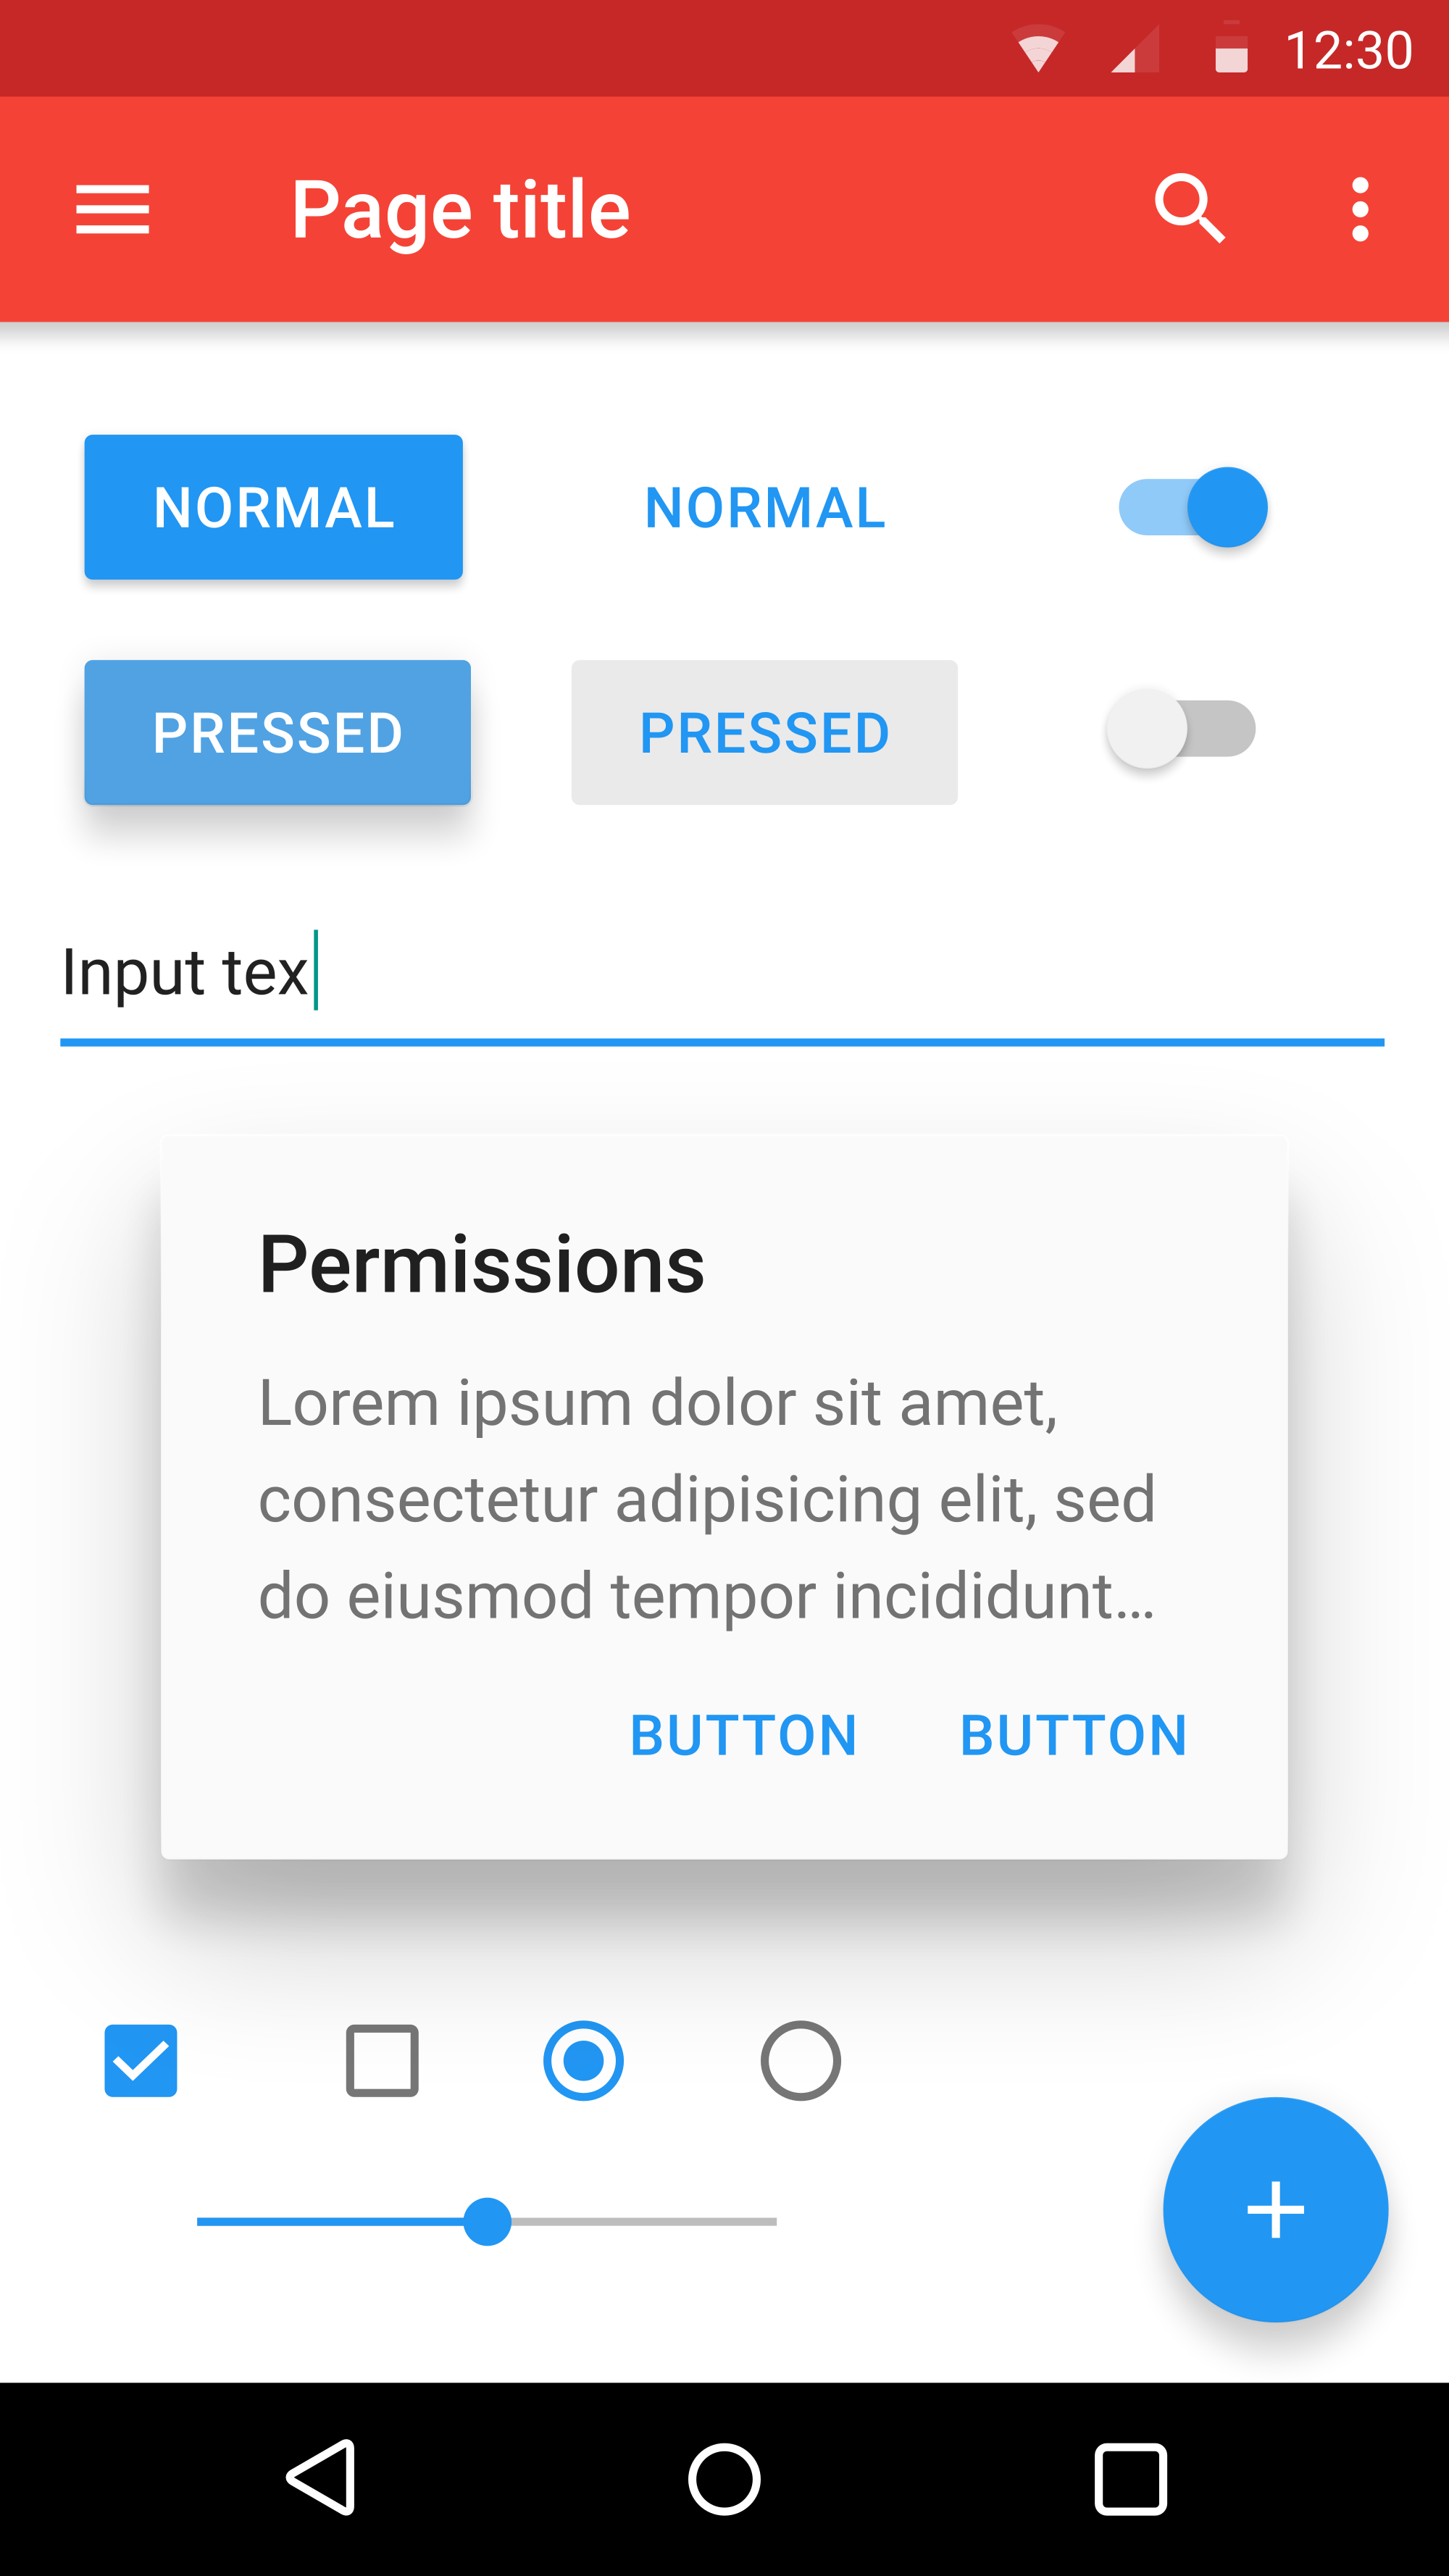
\includegraphics[width=150pt]
    {images/materialdesign.png}
  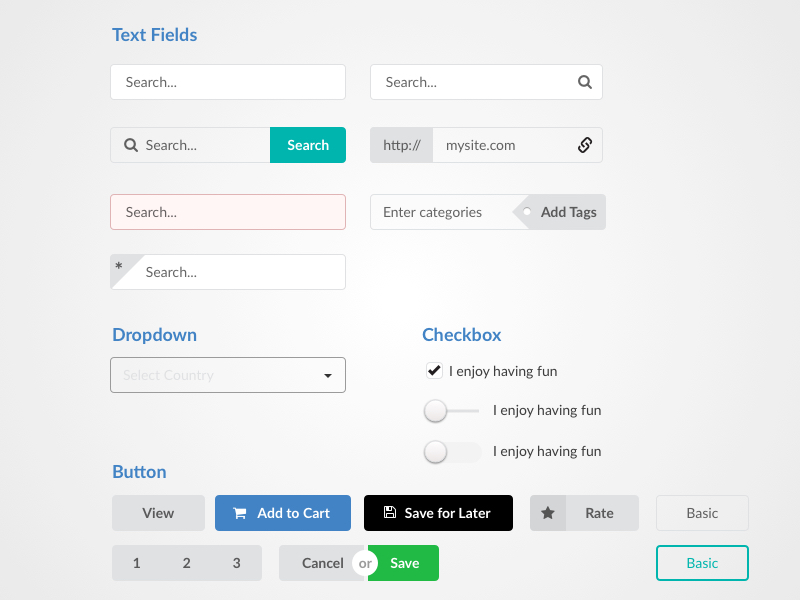
\includegraphics[width=320pt]
    {images/semanticui.jpg}
  \caption{Material Design on a mobile device (left) and Semantic UI components (right). (Source: https://wikipedia.org, https://www.sketchappsources.com/)}
\end{figure}

We pick Semantic UI and its React implementation.
